% Template for ICIP-2015 paper; to be used with:
%          spconf.sty  - ICASSP/ICIP LaTeX style file, and
%          IEEEbib.bst - IEEE bibliography style file.
% --------------------------------------------------------------------------
\documentclass{article}
\usepackage{spconf,amsmath,graphicx}

% Example definitions.
% --------------------
\def\x{{\mathbf x}}
\def\L{{\cal L}}

% Title.
% ------
\title { Deep convolution networks for large scale image classification - A Survey  }
%
% Single address.
% ---------------
\name{Author(s) Name(s)\thanks{Thanks to XYZ agency for funding.}}
\address{Author Affiliation(s)}
%
% For example:
% ------------
%\address{School\\
%	Department\\
%	Address}
%
% Two addresses (uncomment and modify for two-address case).
% ----------------------------------------------------------
%\twoauthors
%  {A. Author-one, B. Author-two\sthanks{Thanks to XYZ agency for funding.}}
%	{School A-B\\
%	Department A-B\\
%	Address A-B}
%  {C. Author-three, D. Author-four\sthanks{The fourth author performed the work
%	while at ...}}
%	{School C-D\\
%	Department C-D\\
%	Address C-D}
%
\begin{document}
%\ninept
%
\maketitle
%
\begin{abstract}
This paper explores the existing learning methods  in the area of image classification.
\end{abstract}
%
\begin{keywords}
One, two, three, four, five
\end{keywords}
%
\section{Introduction}
\label{sec:intro}
Image classification is the process of assigning one or more category label to an image or an image region.
Learning methods will 
These guidelines include complete descriptions of the fonts, spacing, and
related information for producing your proceedings manuscripts. Please follow
them and if you have any questions, direct them 
\texttt{info@icip2015.org}.

\section{Formatting your paper}
\label{sec:format}

All printed material, including text, illustrations, and charts, must be kept
within a print area of 178 mm (7 in.) wide by 229 mm (9 in.) high. Do
not write or print anything outside the print area. The top margin must be 25 mm (1
in.), except for the title page, and the left margin must be 19 mm (0.75 in.).  All {\it text} must be in a two-column format. Columns are to be 86 mm (3.39
in.) wide, with a 6 mm (0.24 in.) space between them. Text must be
fully justified.


\section{Network In Network }
Inspired by the work of Ian J. Goodfellow et al.\cite{Goodfellow2013} on maxout networks,  Min Lin et al.\cite{Lin2013} introduced a micro network in each convolution layer so that it will compute more abstract features.This network gave a state-of-the-art performance in  ILSVRC 2013 competition with an error rate of 12.95\%.





Matthew D. Zeiler and Rob Fergus\cite{Zeiler2013} presented a method to visualize the function of intermediate feature layers of CNNs and used as a diagnostic tool to improve  the model proposed by Krizhevsky et al.\cite{Krizhevsky2012a}. This method helped  them  to understand  activation in the feature maps with respect to the input patterns. It shows Krizhevsky et al.'s architecture does not have  enough mid frequency coverage in the first layer filters and aliasing artifacts caused by  large stride in the first layer convolutions. Authors solved this problems by decreasing filter size to $7\times7$ and reducing stride to 2.This implementation won the  ILSVRC 2013 competition with an error rate of 11.74\%


Instead of using fixed input size in CNNs, Kaiming He et al.\cite{He2014} suggested  the use of a spooling strategy called  spatial pyramid pooling(SPP)\cite{Grauman2005}\cite{1641019} to avoid cropping or warping of  images. It introduced a new layer on top of the convolution layer and perform aggregation  based on Bag-of-Words (BoW) model \cite{Sivic2003}. But the classical back propagation training methods expect layers to have a fixed   size. To overcome this problem author implemented two fixed size networks with shared parameters and switch the network on alternate epochs. This network is trained using a single GeForce GTX Titan GPU with a starting  learning rate of 0.01 and achieved  a less  error rate of 8.06\% on  ILSVRC 2014 data set. 
\par 
This implementation improves the performance of baseline architectures including ZF-5\cite{Zeiler2013} , Convnet \cite{Krizhevsky2012a} and Overfeat-5/7 \cite{Sermanet2013}. Their study shows, accuracy of CNNs will improve on multi-size training, multi-level pooling, and full-image representations. 
%


Christian Szegedy and et al.\cite{Szegedy} proposed a network named GoogLeNet with receptive field(input layer) of size $244\times244$ with the number of layers around 100. Network is trained using asynchronous stochastic gradient descent with 0.9 momentum and fixed learning rate schedule based on  no of epochs 
. Learning procedure took advantage of  model and data-parallelism in a CPU-based cluster environment. This network gave an error rate of  6.67\%  on  ILSVRC 2014 data set. Their result shows that use of existing dense  blocks to  build the sparse structure can improve the  performance of convolutional networks.



Karen Simonyan and Andrew Zisserman \cite{Arge2015} evaluated the effect of network depth in image classification using very small convolution filters. Their deep network architecture comprise of fixed  size input layers , a stack of convolution layers , three Fully-Connected (FC) layers and  5 max-pooling layers for spatial spooling  over a $2 \times 2$ pixel window with stride 2. Hidden layers are modeled using Rectified Linear Units(ReLU)\cite{Nair2010}. On the hardware side, it uses a multi-GPU system with NVIDIA Titan Black GPUs. Network is trained using multinomial logistic regression  based on backpropagation with momentum of 0.9 and  batch size  256.
\par
 In this work authors formed a conclusion that greater depth with small convolution filters and  initialization of certain layers will cause the learning process to converge in less number  of epochs. This model of the convolution network does not differ from the classical architecture proposed by  LeCun et al.\cite{LeCun1998}. But the authors reported a significant improvement in the performance using an increased depth.  This implementation results in a significant improvement in accuracy with  an error rate of  6.8\% in  ILSVRC 2014 of ImageNet.


The latest attempt in image classification with an error 5.98\% in ImageNet data set is reported by  Ren Wu et al.\cite{Wu2015} of Baidu research.They developed an end to end deep learning  system named Deep Image. It uses a highly optimized parallel algorithm  to implement large deep neural network with augmented input data. The network is trained using stochastic gradient decent algorithms (SGD)[ref] on a custom built high performance system comprised of 36 server nodes, each with 2 six-core Intel Xeon E5-2620 processors and 4 NVIDIA Tesla K40m GPUs . System  uses an InfiniBand  network for interconnections. Parallelism strategies used in their network are model-data parallelism and data parallelism.  These methods have been proposed by Alex Krizhevsky \cite{Krizhevsky2014} and Omry Yadan et al.\cite{Yadan2013} for training convolutional neural networks with SGD on a  multiple GPU systems. But it is not easy extend the same strategies to multiple GPU clusters because of the communication overhead. So the  Baidu Team focused on minimizing network data transfers and overlapping the computation. They use butterfly synchronization and lazy update strategies to achieve data parallelism in the gradient computation. Their results show model-data parallelism is better when number of GPUs is less than 16. Implementation of Data parallelism in a large number  of GPU  cluster is better because of the constant communication requirements.
\par
The authors have explored different data augmentation techniques to increase the number of labeled images in the training set. This includes color casting, Vignetting, Lens distortion, Rotation, Flipping, and  Cropping. Instead of using the same resolution on all images, they have trained separate models at different scales, combined results by averaging soft max class posteriors.
Data set used in this experiment was subset of ImageNet dataset, used in the competition ImageNet Large-Scale Visual Recognition Challenge (ILSVRC)\cite{Berg2010}. This data set includes 1.2 million images which contain 1,000 categories.
\par
 Major contribution of this work is the demonstration of tremendous computational power to achieve high accuracy in image classification.
It also shows augmented multi-scale images can be combined to achieve less error rate in convolutional network in the context of the image classification. 






\section{PAGE TITLE SECTION}
\label{sec:pagestyle}

The paper title (on the first page) should begin 35 mm (1.38 in.) from the
top edge of the page, centered, completely capitalized, and in Times 12-point,
boldface type. The authors' name(s) and affiliation(s) appear below the title
in capital and lower case letters. Papers with multiple authors and
affiliations may require two or more lines for this information. Please note
that papers should not be submitted blind; include the authors' names on the
PDF.

\section{TYPE-STYLE AND FONTS}
\label{sec:typestyle}

To achieve the best rendering both in printed proceedings and electronic proceedings, we
strongly encourage you to use Times-Roman font. In addition, this will give
the proceedings a more uniform look. Use a font that is no smaller than nine
point type throughout the paper, including figure captions.

In nine point type font, capital letters are 2 mm high. {\bf If you use the
smallest point size, there should be no more than 3.2 lines/cm (8 lines/in.)
vertically.} This is a minimum spacing; 2.75 lines/cm (7 lines/in.) will make
the paper much more readable. Larger type sizes require correspondingly larger
vertical spacing. Please do not double-space your paper. TrueType or
Postscript Type 1 fonts are preferred.

The first paragraph in each section should not be indented, but all the
following paragraphs within the section should be indented as these paragraphs
demonstrate.

\section{MAJOR HEADINGS}
\label{sec:majhead}

Major headings, for example, ``1. Introduction'', should appear in all capital
letters, bold face if possible, centered in the column, with one blank line
before, and one blank line after. Use a period (``.'') after the heading number,
not a colon.

\subsection{Subheadings}
\label{ssec:subhead}

Subheadings should appear in lower case (initial word capitalized) in
boldface. They should start at the left margin on a separate line.
 
\subsubsection{Sub-subheadings}
\label{sssec:subsubhead}

Sub-subheadings, as in this paragraph, are discouraged. However, if you
must use them, they should appear in lower case (initial word
capitalized) and start at the left margin on a separate line, with paragraph
text beginning on the following line.  They should be in italics.

\section{PAPER FORMAT}
\label{sec:print}

Format you paper for US letter, $8.5 \times 11$-in. paper.
A4 paper is also acceptable, but please leave the extra 0.5 inch (12 mm)
empty at the BOTTOM of the page and follow the top and left margins as
specified. If the last page of your paper is only partially filled, arrange
the columns so that they are evenly balanced if possible, rather than having
one long column.

In LaTeX, to start a new column (but not a new page) and help balance the
last-page column lengths, you can use the command ``$\backslash$pagebreak'' as
demonstrated on this page (see the LaTeX source below).

\section{PAGE NUMBERING}
\label{sec:page}

Please do {\bf not} paginate your paper. Page numbers, session numbers, and
conference identification will be inserted when the paper is included in the
proceedings.

\section{ILLUSTRATIONS, GRAPHS, AND PHOTOGRAPHS}
\label{sec:illust}

Illustrations must appear within the designated margins. They may span the two
columns. If possible, position illustrations at the top of columns, rather
than in the middle or at the bottom.  Caption and number every illustration.
All halftone illustrations must be clear black and white prints. Colors may be
used, but they should be selected so as to be readable when printed on a
black-only printer.

Since there are many ways, often incompatible, of including images (e.g., with
experimental results) in a LaTeX document, below is an example of how to do
this \cite{Lamp86}.

\section{FOOTNOTES}
\label{sec:foot}

Use footnotes sparingly (or not at all!) and place them at the bottom of the
column on the page on which they are referenced. Use Times 9-point type,
single-spaced. To help your readers, avoid using footnotes altogether and
include necessary peripheral observations in the text (within parentheses, if
you prefer, as in this sentence).

% Below is an example of how to insert images. Delete the ``\vspace'' line,
% uncomment the preceding line ``\centerline...'' and replace ``imageX.ps''
% with a suitable PostScript file name.
% -------------------------------------------------------------------------
\begin{figure}[t]

\begin{minipage}[b]{1.0\linewidth}
  \centering
  \centerline{
\includegraphics[width=8.5cm]{Figures/image1}}
%  \vspace{2.0cm}
  \centerline{(a) Result 1}\medskip
\end{minipage}
%
\begin{minipage}[b]{.48\linewidth}
  \centering
  \centerline{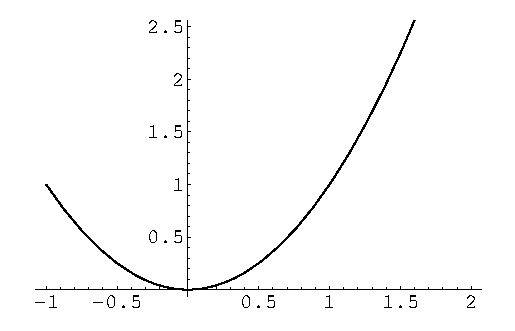
\includegraphics[width=4.0cm]{Figures/image3}}
%  \vspace{1.5cm}
  \centerline{(b) Results 3}\medskip
\end{minipage}
\hfill
\begin{minipage}[b]{0.48\linewidth}
  \centering
  \centerline{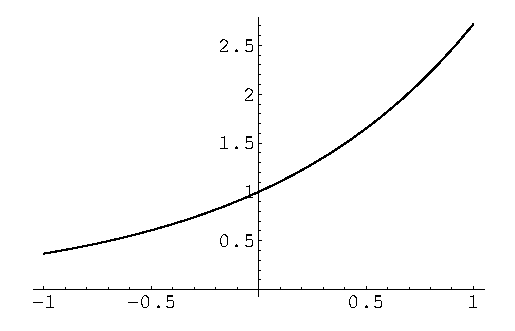
\includegraphics[width=4.0cm]{Figures/image4}}
%  \vspace{1.5cm}
  \centerline{(c) Result 4}\medskip
\end{minipage}
%
\caption{Example of placing a figure with experimental results.}
\label{fig:res}
%
\end{figure}


% To start a new column (but not a new page) and help balance the last-page
% column length use \vfill\pagebreak.
% -------------------------------------------------------------------------
%\vfill
%\pagebreak

\section{COPYRIGHT FORMS}
\label{sec:copyright}

You must include your fully completed, signed IEEE copyright release form when
form when you submit your paper. We {\bf must} have this form before your paper
can be published in the proceedings.

\section{REFERENCES}
\label{sec:ref}

List and number all bibliographical references at the end of the
paper. The references can be numbered in alphabetic order or in
order of appearance in the document. When referring to them in
the text, type the corresponding reference number in square
brackets as shown at the end of this sentence \cite{C2}. An
additional final page (the fifth page, in most cases) is
allowed, but must contain only references to the prior
literature.

% References should be produced using the bibtex program from suitable
% BiBTeX files (here: refs). The IEEEbib.bst bibliography
% style file from IEEE produces unsorted bibliography list.
% -------------------------------------------------------------------------
\bibliographystyle{IEEEbib}
\bibliography{refs}

\end{document}
